\section{Creating Structure}
In previous chapters it was determined that the aim of this paper can be achieved by creating an agent-based framework, and the first step to create a framework is to specify its structure. The current goal is for this structure to model the structure of games. So here is a simple example of a couple of different games from different times.
\par
\textbf{PAC-MAN.} Released in 1980, this simple arcade game is not hard to be described.
The goal is to collect all little yellow dots while avoiding collision with monsters.
\par
\textbf{The Witcher 3.} One of the most complex RPG games released in 2015. Features enormous game world, thousands of characters, and much more assets.
\par
The idea is to take a closer look at this 2 games and try create the optimal classification for their entities. Let us start with the easy one.\par
As simple as it is, PAC-MAN features 3 classes of entities, little yellow dots, monsters, and the PAC-MAN itself. Since we are using agent notion, the next step will be to describe this entities in terms of BDI execution model. Let us start with PAC-MAN. It has at least 1 obvious goal -- to collect all yellow dots. As for its intentions and beliefs, they are determined by the player. Monsters on the other hand have a desire to reach PAC-MAN and individual plans of doing so. It seems like the only entity that is left is the small yellow dot. It has no obvious goals, it is not autonomous, and that lead us to a rational conclusion it should not be represented as an agent. Therefore, we need already create 2 classes of entities. Let us call them \texttt{GameAgent} and \texttt{GameObject}. But there is one more entity. The environment in which all other entities are situated -- the map. In general, the only functions it must have are to contain other objects and provide the means for their execution and communication. But in our case we may combine it with an actual map, featuring walls (because walls can not be influenced by anything) to simplify the structure. The name for this type of entities will be \texttt{GameEnvironment}. At this point the results can be shown in Figure~\ref{PacMan}. \par
 \begin{figure}[h!]
    \begin{center}
      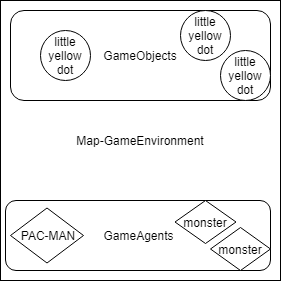
\includegraphics[width=200pt]{PAC-MAN}
      \caption{Agent/Object/Environment structure for PAC-MAN game example.}
      \label{PacMan}
     \end{center}
    \end{figure}
Now let us look how does this simple structure can be applicable to the second game. The \texttt{GameAgent/GameObject} classification mechanism stays the same -- all agents are entities  easier to be described with their beliefs and desires than with algorithms. However, there are entities with the similar functionality to \texttt{GameAgent} or \texttt{GameObject} that encapsulate other agents, as it does \texttt{GameEnvironment}. The obvious example is the house  that is implemented as a single \texttt{GameObject}, but may contain other \texttt{GameAgents} and \texttt{GameObjects} inside. Therefore, each game environment can also be a \texttt{GameObject} or \texttt{GameAgent} in another game environment. Also every \texttt{GameAgent} entity extends \texttt{GameObject}.\texttt{GameAgent} can be described as \texttt{GameObject} with added reasoning mechanism and individual computational power. Class relations are depicted in Figure~\ref{ClassInh}.
 \begin{figure}[h!]
    \begin{center}
      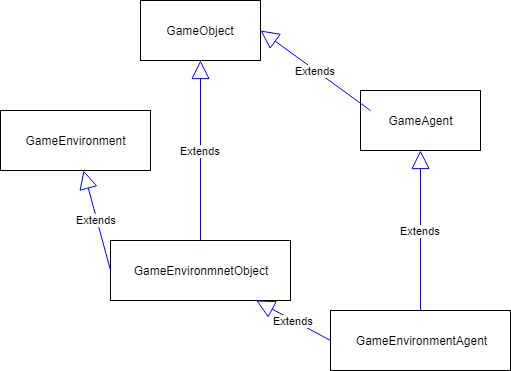
\includegraphics[width=350pt]{game_inheritance}
      \caption{Class inheritance for Model0.}
      \label{ClassInh}
     \end{center}
    \end{figure}
Despite the initialization, there was no specification provided to the classes. The set of already defined classes along with their specifications can be later referenced as \textbf{Model0}.
\begin{center}
    \textbf{Model0 specification}
\end{center}
\subsection{Communication between Model0 entities}
The communication is a process that includes sending data to another structural entity.
The list of possible events that trigger communication mechanisms in GameEnvironment include:
\begin{enumerate}
\item The \texttt{GameAgent} executes an action.This action is the most general one, yet in most games it has a specific meaning. Consider the following situation: you are in the train trying to explain someone a theorem, but all the noises and voices around stop your constantly ruin your attempts to deliver the information to your interlocutor. The environment is responsible for the choice whether your actions succeed or fail to execute. That is why in reality, and, therefore, in most games, each action attempt should be double-checked by the environment itself. Also environment controls whatever response this agent might get afterwards. It requires the communication mechanism between two \texttt{GameAgents} to look similar to the one in Figure~\ref{MessagePass}.
 \begin{figure}[h!]
    \begin{center}
      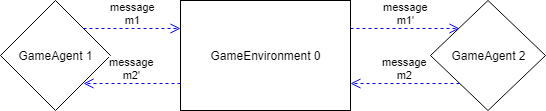
\includegraphics[width=400pt]{agents_message_environment}
      \caption{Message passing example.}
      \label{MessagePass}
     \end{center}
    \end{figure}
If $M$ is the set of all possible messages (including message without data) and $E_i$ is the state of the environment (that includes every information environment possess, including accessible information from its objects), then each message, sent from one object to another one undergoes transformation, specified by a function \(correct: M\times E_i \rightarrow M\).
However, in reality, while processing the message, environment might send and collect several messages from any objects that it contains.
\item The \texttt{GameEnvironment} executes an action. In most games time is one of the global parameters. The responsibility to change time in most cases should be granted to the environment itself to avoid the possibility of loosing or destroying the agent and the following problems. By making \texttt{GameEnvironment} a time-managing entity it becomes a perfect choice for triggering time-specific events. Time-specific events may include creating, destroying, modifying and notifying aggregated entities of the \texttt{GameEnvironment}.

On the other hand, time can be managed by some aggregated entity like a \texttt{GameAgent}, yet , while simplifying \texttt{GameEnvironment's} structure, this design choice might make the overall framework less understandable.
\end{enumerate}

\subsection{GameObject}
 \begin{figure}[p]
    \begin{center}
      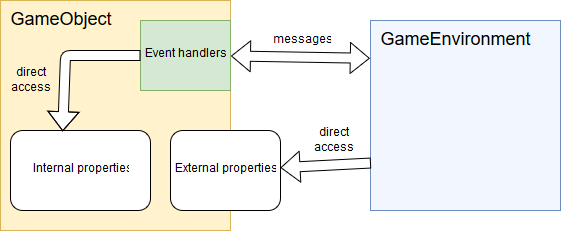
\includegraphics[width=400pt]{GameObject}
      \caption{GameObject structure in Model0.}
      \label{GameObj}
     \end{center}
    \end{figure}
This class (depicted in Figure~\ref{GameObj}) should describe every possible object that have state and can be created, destroyed or changed during the simulation.
Now it is possible to assemble it piece by piece by mapping different examples on PAC-MAN entities, which are mentioned earlier in this chapter.
\begin{itemize}
\item Properties. \par
Each object is defined by its properties.
%In this part we will analyze the properties, that can be saved as a value.
These properties serve as arguments for other objects/agents. For example, each object in PAC-MAN must have its own position. There are two types of properties:
\begin{definition}{External properties}. This kind of properties is directly accessible to the environment (\textit{read}, \textit{modify}, \textit{add} and \textit{remove} permissions), yet can be inaccessible to the containing agent itself. The only way to to perform any direct access action (\textit{read}, \textit{modify}, \textit{add} or \textit{remove}) for the agent is to send a message request to the environment.
 \end{definition}
\begin{definition}{Internal properties.} These properties can be inaccessible to the environment, but must be directly accessible to the agent itself. For example, if a box contains an apple, environment has no need to know what is it in the box until it is opened. When the box is opened and the insides of the box becomes an external property, environment can decide whether the apple could be in the box and, if it violates some of the rules, simply deny it.
 \end{definition}
\item Event handlers
\begin{definition}{Event handlers.} 
These handlers are responsible for responses of the \texttt{GameObject} to external messages that are created within the \texttt{GameEnvironment}. For example, when someone tries to fire a gun, the corresponding event handler of a gun would determine the appearance and the direction of the bullet.
\end{definition}
\end{itemize}
\subsection{GameAgent}
  \begin{figure}[p]
    \begin{center}
      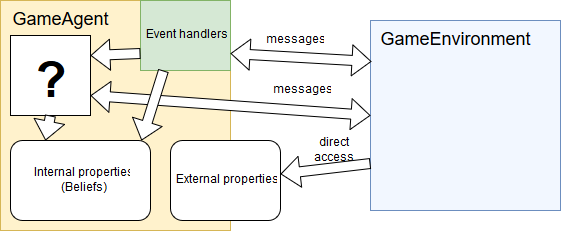
\includegraphics[width=400pt]{GameAgent}
      \caption{GameAgent structure in Model0.}
      \label{GameAg}
     \end{center}
    \end{figure}
\texttt{GameAgent} (depicted in Figure~\ref{GameAg}) features all the structural details from the \texttt{GameObject} class.
External properties have the same specification. However, internal properties are also used to contain agent's belief structure, so it will be easier to refer to them as beliefs or the internal state. At this point, internal structure of a \texttt{GameAgent} may remain undefined. However, since there should be some way for communication with environment, \texttt{GameAgent} must be given a \texttt{GameEnvironment} upon aggregation.

\subsection{GameEnvironment}
 \begin{figure}[p]
    \begin{center}
      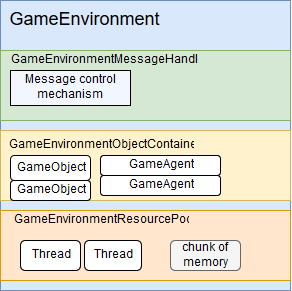
\includegraphics[width=250]{GameEnvironment}
      \caption{GameEnvironment structure in Model0.}
      \label{GameEnv}
     \end{center}
    \end{figure}
The \texttt{GameEnvironment} class (depicted in Figure~\ref{GameEnv}) is the least clearly specified. For example, in the PAC-MAN model it was used to represent some of the most simple objects (maze blocks). The pure \texttt{GameEnvironment} class consists of \texttt{GameEnvironmentMessageHandler}, \texttt{GameEnvironmentObjectContainer} and \texttt{GameEnvironmentResourcePool}, each of which executing its own functions.
\begin{itemize}
\item \textbf{GameEnvironmentMessageHandler} is responsible for message control. It receives messages, determines how to change them (based on a set of rules it is given) and who should receive them. The mechanism of changing messages gives the \texttt{GameEnvironment} a complete control over agent interactions within the \texttt{GameEnvironment}.
\item \textbf{GameEnvironmentObjectContainer} is responsible for containing objects. Its functions may include distributing memory as well as computational power between entities. It also should make it possible to dynamically create and to destroy entities.
\item \textbf{GameEnvironmentResourcePool} is a container for resources that are given to the environment.
\end{itemize}
\subsection{GameEnvironmentObject/GameEnvironmentAgent}
These are the most complex classes in \textit{Model0}. The goal of these classes is to provide an ability of creating a recursive depth in the system by creating the \texttt{GameObject} or \texttt{GameAgent} that also includes \texttt{GameEnvironment} functionality. The \texttt{GameEnvironment} that contain \texttt{GameEnvironmentObject} (or \texttt{GameEnvironmentAgent}) is called external environment. The \texttt{GameEnvironment} that is a part of the describable entity is called internal environment. The described classes behave similarly to the \texttt{GameEnvironment} class but also feature the unique subclass, \texttt{GameDoubleAgent}, or \texttt{GameDoubleObject} respectively. This class differs from \texttt{GameObject} (or \texttt{GameAgent}) in ability to send messages to both internal and external environment. The feature creates a connection that can be used to pass data between environments.\par

